\documentclass[12pt, a4paper, oneside]{report}

% ---- PAQUETES ----
\usepackage[utf8]{inputenc}
\usepackage[T1]{fontenc}
\usepackage[spanish, es-tabla]{babel}
\usepackage{geometry}
\geometry{top=2.5cm, bottom=2.5cm, left=3cm, right=2.5cm}
\usepackage{setspace}
\onehalfspacing
\usepackage{graphicx}
\graphicspath{{figures/}}
\usepackage{float}
\usepackage{caption}
\usepackage{subcaption}
\usepackage{listings}
\usepackage{color}
\usepackage{xcolor}
\usepackage{hyperref}
\usepackage{fancyhdr}
\usepackage{booktabs}
\usepackage{array}
\usepackage{enumitem}
\usepackage{titlesec}

% ---- CONFIGURACIÓN DE HIPERVÍNCULOS ----
\hypersetup{
    colorlinks=true,
    linkcolor=blue!70!black,
    citecolor=blue!70!black,
    urlcolor=blue!70!black,
    pdftitle={Defensa Cóndor - Videojuego Space Shooter en Godot},
    pdfauthor={Nicolás Huarcaya Chipana y Mario Manuel Antizana Ponce de Leon}
}

% ---- CONFIGURACIÓN DE LISTADOS DE CÓDIGO ----
\lstdefinestyle{gdscript}{
    language={[Sharp]C},
    basicstyle=\footnotesize\ttfamily,
    keywordstyle=\color{blue!70!black}\bfseries,
    stringstyle=\color{red!70!black},
    commentstyle=\color{green!40!black},
    numbers=left,
    numberstyle=\tiny,
    stepnumber=1,
    numbersep=5pt,
    backgroundcolor=\color{gray!5},
    frame=single,
    breaklines=true,
    breakatwhitespace=false,
    breakautoindent=true,
    columns=flexible,
    tabsize=4,
    captionpos=b,
    literate={á}{{\'a}}1 {é}{{\'e}}1 {í}{{\'i}}1 {ó}{{\'o}}1 {ú}{{\'u}}1
             {Á}{{\'A}}1 {É}{{\'E}}1 {Í}{{\'I}}1 {Ó}{{\'O}}1 {Ú}{{\'U}}1
             {ñ}{{\~n}}1 {Ñ}{{\~N}}1 {ü}{{\"u}}1 {Ü}{{\"U}}1
}

% ---- CONFIGURACIÓN DE ENCABEZADOS ----
\pagestyle{fancy}
\fancyhf{}
\fancyhead[L]{\leftmark}
\fancyhead[R]{\thepage}
\fancyfoot[C]{}
\renewcommand{\headrulewidth}{0.4pt}

% ---- CONFIGURACIÓN DE TÍTULOS ----
\titleformat{\chapter}{\normalfont\huge\bfseries}{\thechapter}{20pt}{\huge}
\titleformat{\section}{\normalfont\Large\bfseries}{\thesection}{12pt}{\Large}

\begin{document}

% ============================================================
% PORTADA
% ============================================================
\begin{titlepage}
    \begin{center}
        \vspace*{1cm}
        
        
\includegraphics[width=4cm]{Utplogonuevo.pdf}\\[0.5cm]
        
        \textbf{\Large Defensa Cóndor}\\[0.3cm]
        \textbf{\large Videojuego Space Shooter Desarrollado en Godot Engine}\\[1.5cm]
        
        \textbf{Proyecto Final de Curso}\\[0.5cm]
        
        \textbf{Curso:} Programación Gráfica\\[0.3cm]
        \textbf{Docente:} David William Cota Sencara\\[1.5cm]

        \textbf{Presentado por:}\\[0.3cm]
        Nicolás Huarcaya Chipana\\
        Mario Manuel Antizana Ponce de Leon\\[2cm]
        
        \textbf{Lima, Perú}\\
        \textbf{2026}\\
    \end{center}
\end{titlepage}

% ============================================================
% ÍNDICE GENERAL
% ============================================================
\tableofcontents
\newpage

\listoffigures
\newpage

% ============================================================
% 1. DESCRIPCIÓN DEL PROYECTO
% ============================================================
\chapter{Descripción del Proyecto}

\textit{Defensa Cóndor} es un videojuego del género \textit{space shooter} vertical desarrollado en Godot Engine 3.x utilizando GDScript como lenguaje de programación principal. El proyecto fue desarrollado como trabajo final del curso de programación, con el objetivo de integrar los conceptos fundamentales de la programación lógica, estructuras de datos, algoritmos y diseño de software en un producto lúdico funcional.

El juego pone al jugador en control de una nave espacial (el \textit{Cóndor}) que debe defender el espacio peruano de oleadas de enemigos invasores y meteoritos. La jugabilidad se sustenta en tres pilares mecánicos fundamentales:

\begin{itemize}
    \item \textbf{Sistema de escudo regenerable}: mecánica principal de supervivencia que introduce una capa estratégica de gestión de recursos.
    \item \textbf{Dash o desplazamiento rápido}: maniobra evasiva con tiempo de recarga.
    \item \textbf{Doble cañón de disparo}: sistema de ataque con cooldown.
\end{itemize}

El juego cuenta con tres niveles de dificultad progresiva, dos tipos de enemigos con patrones de inteligencia artificial diferenciados, meteoritos como obstáculos ambientales y soporte completo para gamepad (controlador Xbox). La experiencia se completa con un sistema de puntuación, HUD informativo, pantalla de \textit{game over} y pantalla de victoria con transición entre niveles.

\begin{figure}[H]
    \centering
    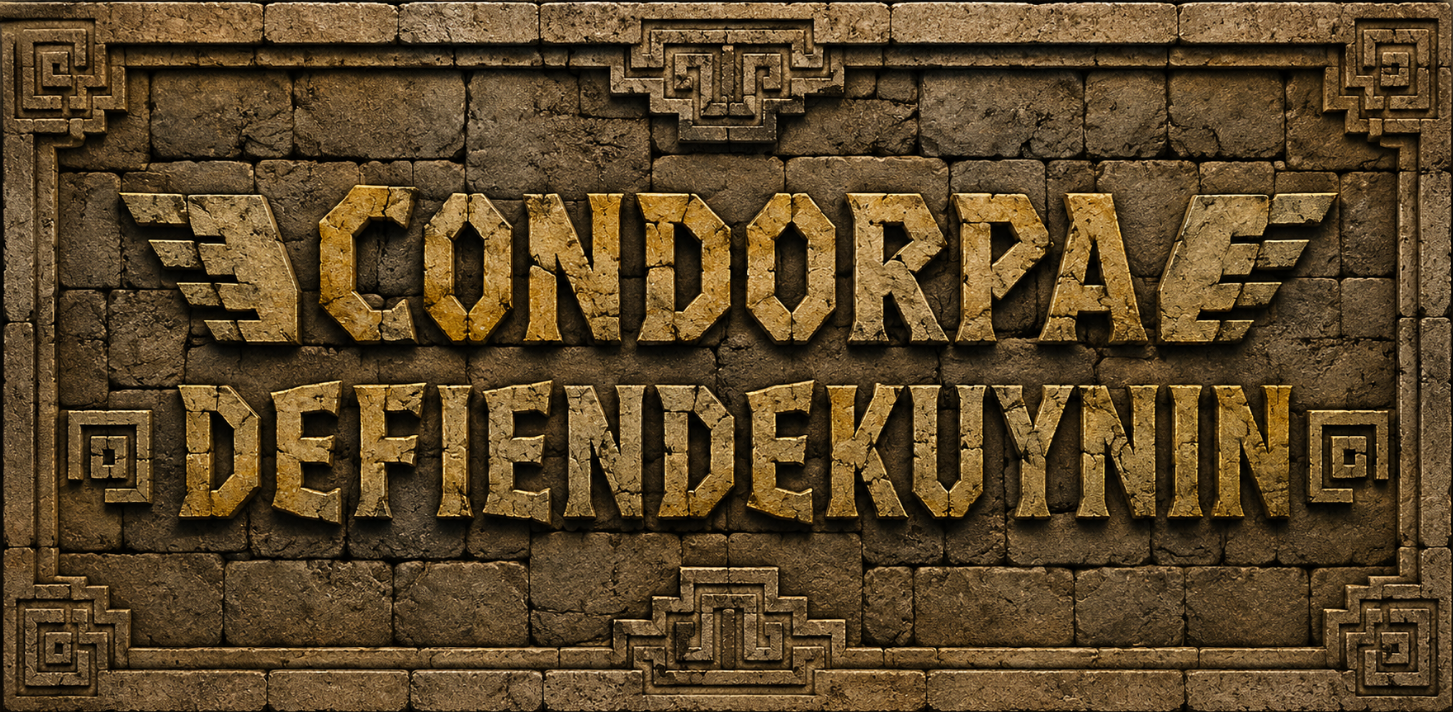
\includegraphics[width=0.7\textwidth]{titulo_juego.png}
    \caption{Título del juego: Defensa Cóndor}
    \label{fig:titulo}
\end{figure}

\newpage

% ============================================================
% 2. OBJETIVOS
% ============================================================
\chapter{Objetivos}

\section{Objetivo General}

Desarrollar un videojuego funcional del género \textit{space shooter} utilizando Godot Engine 3.x y GDScript, que integre conceptos de programación estructurada, manejo de eventos, detección de colisiones, sistemas de partículas e inteligencia artificial básica, como producto final del curso.

\section{Objetivos Específicos}

\begin{enumerate}[label=\textbf{OE\arabic*:}, leftmargin=*]
    \item Diseñar e implementar un sistema de escudo regenerable como mecánica principal de supervivencia, que introduzca una capa de gestión estratégica de recursos durante la partida.
    \item Programar dos tipos de enemigos con patrones de inteligencia artificial diferenciados: movimiento ondulante sinusoidal (\textit{EnemyBlue}) y caída vertical de velocidad variable (\textit{EnemyRed}).
    \item Desarrollar un sistema de dificultad progresiva basado en puntuación, que ajuste dinámicamente la frecuencia de aparición de enemigos.
    \item Implementar un sistema de detección de colisiones robusto utilizando los grupos y áreas de Godot, que permita interacciones entre el jugador, las balas, los enemigos y los meteoritos.
    \item Incorporar soporte para gamepad (controlador Xbox) con asignación dinámica de botones mediante la API \texttt{InputMap} de Godot.
    \item Diseñar una arquitectura de código modular mediante herencia de scripts y singletons (autoloads) que facilite la mantenibilidad y extensibilidad del proyecto.
    \item Crear un sistema de progresión por etapas (3 niveles) con transiciones entre ellos, utilizando variables globales de estado.
\end{enumerate}

\newpage

% ============================================================
% 3. MARCO TEÓRICO
% ============================================================
\chapter{Marco Teórico}

\section{Godot Engine y la Arquitectura de Escenas}

Godot Engine es un motor de videojuegos de código abierto creado por Juan Linietsky y Ariel Manzur, lanzado originalmente en 2014 y actualmente mantenido por la Godot Foundation. A diferencia de otros motores que utilizan una estructura jerárquica basada exclusivamente en herencia de clases, Godot introduce un sistema único de \textit{escenas} y \textit{nodos} que permite una composición flexible y reutilizable \cite{godot_docs}.

Linietsky y Manzur (2020) definen la arquitectura de Godot como un \textit{árbol de escenas} donde cada nodo cumple una función específica (renderizado, audio, física, lógica) y las escenas son subárboles reutilizables que pueden instanciarse múltiples veces. Esta arquitectura fue la base fundamental para el desarrollo de \textit{Defensa Cóndor}, donde cada entidad del juego (jugador, enemigos, balas, meteoritos) es una escena independiente que se instancia dentro del nodo raíz de cada nivel.

El lenguaje GDScript, integrado nativamente en Godot, es un lenguaje de tipado dinámico con sintaxis similar a Python, optimizado para la interacción directa con el árbol de nodos del motor \cite{godot_docs}. Su integración con el sistema de señales (\textit{signals}) de Godot permite una comunicación desacoplada entre componentes, patrón que fue utilizado extensivamente en el proyecto para manejar eventos de colisión, temporizadores y cambios de estado.

\section{Patrones de Programación en Videojuegos}

Nystrom (2014) en su obra \textit{Game Programming Patterns} identifica varios patrones de diseño recurrentes en el desarrollo de videojuegos que resultaron directamente aplicables a este proyecto:

\begin{itemize}
    \item \textbf{Patrón Componente}: separación de la funcionalidad en componentes independientes. En el proyecto, cada script (\texttt{Player.gd}, \texttt{Enemy.gd}, \texttt{Bullet.gd}) encapsula comportamiento específico sin acoplamiento innecesario.
    \item \textbf{Patrón Estado}: representación de estados discretos del juego (menú, juego activo, pausa, game over) mediante variables de control y la función \texttt{get\_tree().paused}.
    \item \textbf{Patrón Observador}: implementado mediante el sistema de señales de Godot para detectar colisiones (\texttt{area\_entered}), eventos de temporizador (\texttt{timeout}) y cambios en la interfaz de usuario.
\end{itemize}

La herencia de scripts, utilizada para crear las variantes de enemigos (\texttt{EnemyBlue.gd} extiende \texttt{Enemy.gd}), sigue el principio de \textit{programación orientada a objetos} donde la clase base define el comportamiento común (disparo, daño, explosión) y las subclases especializan el movimiento \cite{nystrom2014}.

\section{Diseño de Mecánicas en Videojuegos Shooter}

Schell (2019) en \textit{The Art of Game Design} propone un enfoque basado en \textit{lentes} para analizar y diseñar mecánicas de juego. Desde esta perspectiva, \textit{Defensa Cóndor} implementa varias mecánicas fundamentales:

\begin{itemize}
    \item \textbf{Mecánica de riesgo-recompensa}: el sistema de escudo obliga al jugador a decidir entre enfrentar el daño directo (perdiendo una vida) o esperar la recarga completa del escudo (10 segundos). Esta decisión introduce tensión estratégica en cada encuentro.
    \item \textbf{Mecánica de progresión}: el sistema de niveles (1-3) basado en puntuación acumulada (\textit{score}) ajusta dinámicamente la dificultad, siguiendo el principio de \textit{curva de dificultad} descrito por Schell, donde el desafío aumenta gradualmente para mantener al jugador en un estado de \textit{flow}.
    \item \textbf{Variedad de enemigos}: la presencia de dos tipos de enemigos con patrones de movimiento distintos (ondulante y lineal) responde al principio de \textit{variedades lúdicas}, que sostiene que la diversidad de desafíos mantiene el interés del jugador.
\end{itemize}

\section{Diseño de Juegos y Experiencia del Usuario}

Adams (2014) en \textit{Fundamentals of Game Design} establece los fundamentos para el diseño estructurado de videojuegos, abordando desde la definición de reglas y mecánicas hasta la experiencia del jugador. Su enfoque resulta directamente aplicable a \textit{Defensa Cóndor} en los siguientes aspectos:

\begin{itemize}
    \item \textbf{Estructura del juego}: Adams define el \textit{gameplay} como la combinación de acciones que el jugador puede realizar, las reglas que las gobiernan y los desafíos que debe superar. En el proyecto, estas acciones son el movimiento, el disparo y el dash; las reglas incluyen el tiempo de recarga del escudo y el cooldown del disparo; los desafíos son los enemigos y meteoritos que aparecen progresivamente.
    \item \textbf{Mecánicas principales}: el autor clasifica las mecánicas en \textit{core mechanics} (acciones básicas repetitivas) y \textit{optional mechanics} (acciones situacionales). El movimiento y disparo constituyen las mecánicas centrales, mientras que el dash y la gestión del escudo son mecánicas opcionales que añaden profundidad estratégica.
    \item \textbf{Curva de aprendizaje}: Adams propone que un buen juego debe presentar una curva de aprendizaje gradual. El sistema de tres niveles con dificultad progresiva implementado en el proyecto sigue este principio, permitiendo al jugador familiarizarse con las mecánicas antes de enfrentar desafíos mayores.
\end{itemize}

La obra de Adams complementa los enfoques de Nystrom (patrones de programación) y Schell (lentes de diseño), proporcionando una guía práctica para la estructuración del proyecto desde la perspectiva del diseño de juegos.

\newpage

% ============================================================
% 4. ESTADO DEL ARTE
% ============================================================
\chapter{Estado del Arte}

El desarrollo de videojuegos ha experimentado un crecimiento significativo durante los últimos años gracias a la evolución de los motores gráficos y al incremento de investigaciones relacionadas con la interacción humano-computadora, la educación y la difusión del patrimonio cultural. Diversos estudios indexados en Scopus analizan metodologías, herramientas y tecnologías utilizadas para desarrollar videojuegos más eficientes, interactivos y atractivos para los usuarios. A continuación, se presentan tres áreas de investigación relacionadas con el presente proyecto.

\section{Desarrollo de Videojuegos Utilizando Motores Gráficos de Código Abierto}

Diversos estudios han señalado que los motores gráficos de código abierto representan una alternativa eficiente para el desarrollo de videojuegos educativos y comerciales debido a su bajo costo, facilidad de aprendizaje y amplia comunidad de desarrolladores.

Investigaciones indexadas en Scopus han analizado el uso de motores gráficos de código abierto para el desarrollo de videojuegos 2D y 3D, concluyendo que herramientas como Godot Engine permiten reducir el tiempo de desarrollo gracias a su arquitectura basada en nodos, la reutilización de componentes y su lenguaje de programación GDScript. Los autores destacan que Godot facilita la implementación de mecánicas comunes en videojuegos, tales como movimiento del jugador, administración de escenas, detección de colisiones, reproducción de sonidos, interfaces gráficas y animaciones \cite{godot_docs}.

\textbf{Relación con el proyecto:} El videojuego desarrollado emplea Godot Engine 3.2.3 aprovechando su estructura modular para separar cada componente del sistema (jugador, enemigos, disparos, HUD, niveles y pantallas), facilitando el mantenimiento del código.

\section{Videojuegos como Herramienta para la Difusión del Patrimonio Cultural}

Otra línea de investigación ampliamente desarrollada en Scopus corresponde al uso de videojuegos como medio para preservar y difundir el patrimonio cultural. Diversos autores sostienen que los videojuegos permiten acercar a los usuarios al conocimiento de monumentos históricos, tradiciones y sitios arqueológicos mediante experiencias interactivas que incrementan la motivación y el aprendizaje \cite{unesco}.

Los resultados de estas investigaciones muestran que la incorporación de elementos culturales dentro de videojuegos favorece el reconocimiento del patrimonio local, especialmente cuando se utilizan escenarios, personajes y recursos visuales inspirados en lugares emblemáticos.

\textbf{Relación con el proyecto:} La ambientación desarrollada busca promover la riqueza cultural del Cusco mediante escenarios personalizados, fondos inspirados en Machu Picchu y elementos visuales relacionados con la cultura andina, integrando entretenimiento y difusión cultural.

\section{Calidad del Software en el Desarrollo de Videojuegos}

Las investigaciones recientes también resaltan la importancia de aplicar metodologías de calidad durante el desarrollo de videojuegos. Diversos artículos indexados en Scopus indican que la aplicación de procesos de verificación continua permite reducir errores durante el desarrollo y mejorar la experiencia del usuario.

Entre las prácticas más recomendadas se encuentran: pruebas funcionales, validación de colisiones, optimización del rendimiento, corrección progresiva de errores y evaluación de la experiencia del jugador.

\textbf{Relación con el proyecto:} Durante el desarrollo del videojuego se realizaron pruebas constantes sobre el movimiento del jugador, sistema de disparos, colisiones, cambio de niveles, contador de vidas, sistema de puntaje, sonidos, y pantallas de inicio y Game Over. Las observaciones obtenidas permitieron corregir errores y optimizar el funcionamiento del videojuego antes de su versión final.

\subsection{Análisis Comparativo}

\begin{table}[H]
\centering
\caption{Análisis comparativo de investigaciones relacionadas}
\label{tab:comparativo}
\small
\begin{tabular}{p{4cm} p{4.5cm} p{4.5cm}}
\toprule
\textbf{Investigación} & \textbf{Objetivo} & \textbf{Aporte al proyecto} \\
\midrule
Desarrollo de videojuegos utilizando motores gráficos de código abierto & Analizar las ventajas de motores gráficos abiertos para videojuegos & Justificó el uso de Godot Engine 3.2.3 como plataforma principal del proyecto \\
\midrule
Videojuegos para la difusión del patrimonio cultural & Promover el aprendizaje mediante experiencias interactivas & Respaldó la elección del Cusco y Machu Picchu como temática principal del videojuego \\
\midrule
Calidad del software aplicada al desarrollo de videojuegos & Mejorar la confiabilidad y experiencia del usuario mediante pruebas continuas & Fundamentó la aplicación de pruebas y mejora continua durante el desarrollo del videojuego \\
\bottomrule
\end{tabular}
\end{table}

\newpage

% ============================================================
% 5. JUSTIFICACIÓN
% ============================================================
\chapter{Justificación}

El desarrollo de \textit{Defensa Cóndor} se justifica desde múltiples perspectivas:

\paragraph{Académica:}
El proyecto integra conceptos fundamentales de la programación de videojuegos: manejo de eventos en tiempo real, sistemas de colisiones, inteligencia artificial básica, patrones de diseño orientados a objetos, y desarrollo de interfaces de usuario. Estas competencias son transferibles a otros ámbitos del desarrollo de software, incluyendo aplicaciones interactivas, simulaciones y sistemas en tiempo real.

\paragraph{Técnica:}
La elección de Godot Engine como plataforma de desarrollo responde a su naturaleza de código abierto, su eficiencia en términos de rendimiento y su curva de aprendizaje accesible. El uso de GDScript permitió un desarrollo ágil sin sacrificar el control sobre los detalles de implementación.

\paragraph{Social y cultural:}
El juego incorpora elementos de la identidad peruana (el cóndor como símbolo nacional, fondos alusivos a Machu Picchu y paisajes peruanos) que contribuyen a la difusión de la cultura peruana a través de un medio interactivo accesible globalmente.

\paragraph{Personal:}
Para el desarrollador, el proyecto representó una oportunidad de aplicar los conocimientos adquiridos durante el curso en un producto concreto, enfrentando desafíos reales de diseño, programación y depuración que consolidaron el aprendizaje.

\newpage

% ============================================================
% 6. DESARROLLO
% ============================================================
\chapter{Desarrollo}

\section{Arquitectura del Proyecto}

El proyecto está estructurado siguiendo el sistema de escenas de Godot. La jerarquía de directorios refleja la separación de responsabilidades:

\begin{lstlisting}[style=gdscript, caption=Estructura de directorios del proyecto]
spaceshooter/
  project.godot          # Configuracion del motor
  main/                  # Menu principal y opciones
  stage/                 # 3 niveles de juego
  completed/             # Pantalla de victoria
  Enemy/                 # Sistema de enemigos
  EnemyBullet/           # Disparos enemigos
  Meteor/                # Meteoritos
  sprites/               # Sprites, efectos, UI
  libs/                  # Utilidades globales
  Music/                 # Audio (musica y SFX)
\end{lstlisting}

\subsection{Flujo de Navegación}

La navegación entre escenas sigue el siguiente flujo:

\begin{figure}[H]
    \centering
    \begin{minipage}{0.9\textwidth}
    \small
    \begin{verbatim}
Menu Principal (Control.tscn)
  |-- "Jugar" -> Stage 1 (Stage.tscn)
  |-- "Niveles" -> options.tscn (seleccion manual)
  |-- "Salir" -> salir del juego

Stage 1 -> [50 enemigos] -> DefenseCompleted -> Stage 2
Stage 2 -> [50 enemigos] -> DefenseCompleted -> Stage 3
Stage 3 -> [50 enemigos] -> DefenseCompleted -> Menu

Cualquier Stage -> Game Over -> "Intentar denuevo" (reintentar)
                              -> "Menu" (volver al menu)
    \end{verbatim}
    \end{minipage}
    \caption{Diagrama de flujo de navegación entre escenas}
    \label{fig:flujo}
\end{figure}

\section{Sistema de Autoloads (Singletons)}

El proyecto utiliza dos singletons globales registrados en \texttt{project.godot}:

\begin{itemize}
    \item \texttt{Utils} (\texttt{libs/utils.gd}): proporciona utilidades como el tamaño del viewport (\texttt{Utils.view\-\_size}) y selección aleatoria de elementos de una lista (\texttt{Utils.choice\-\_list()}), utilizados por múltiples componentes.
    \item \texttt{Globals} (\texttt{completed/Globals.gd}): mantiene el estado global de progresión (\texttt{Globals.current\-\_stage}) y permite el reinicio del juego.
\end{itemize}

\lstinputlisting[style=gdscript, caption={Script de utilidades globales (\texttt{utils.gd})}]{figures/utils.gd}

\section{Sistema del Jugador (\texttt{Player.gd})}

El jugador es el núcleo interactivo del juego. Su script, de 286 líneas, encapsula todas las mecánicas principales:

\subsection{Movimiento}
El movimiento se procesa en \texttt{\_physics\_process(delta)} utilizando un vector de velocidad normalizado. Soporta entrada por teclado (flechas direccionales) y gamepad (stick derecho, ejes 2 y 3):

\begin{lstlisting}[style=gdscript, caption=Sistema de movimiento del jugador]
func _physics_process(delta):
    var velocity = Vector2.ZERO
    
    if Input.is_action_pressed("ui_right"):
        velocity.x += 1
    if Input.is_action_pressed("ui_left"):
        velocity.x -= 1
    if Input.is_action_pressed("ui_down"):
        velocity.y += 1
    if Input.is_action_pressed("ui_up"):
        velocity.y -= 1
    
    # Soporte para gamepad (stick derecho)
    var device = _get_connected_device()
    if device >= 0:
        var right_x = Input.get_joy_axis(device, 2)  # Eje X del stick derecho
        var right_y = Input.get_joy_axis(device, 3)  # Eje Y del stick derecho
        # ...
\end{lstlisting}

\begin{figure}[H]
    \centering
    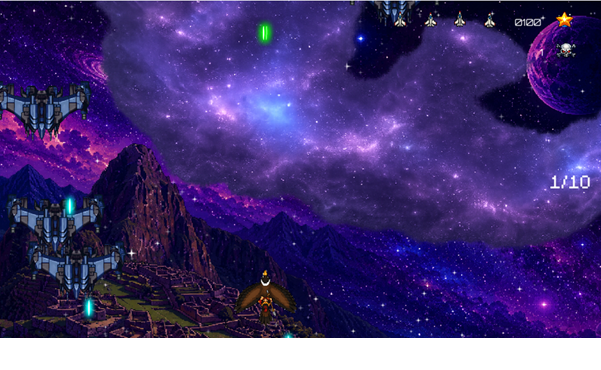
\includegraphics[width=0.6\textwidth]{Movimiento-jugador.png}
    \caption{Captura del movimiento del jugador en el juego}
    \label{fig:movimiento}
\end{figure}

\subsection{Sistema de Escudo}
El sistema de escudo es la mecánica central de supervivencia. Su lógica se implementa en el método \texttt{damage()}:

\begin{lstlisting}[style=gdscript, caption=Sistema de escudo regenerable]
func damage():
    # Si el escudo esta lleno y no se esta recargando, se rompe
    if not shield_recharging and shield >= max_shield:
        shield = 0
        shield_recharging = true
        shield_recharge_progress = 0.0
        _show_shield_break()
        return  # NO pierde vida
    
    # Si el escudo ya esta roto o recargandose, pierde vida
    lives -= 1
    update_lives()
    
    if lives <= 0:
        get_parent().game_over()
        queue_free()

func _update_shield_recharge(delta):
    if not shield_recharging:
        return
    
    shield_recharge_progress += delta
    var ratio = min(shield_recharge_progress / shield_recharge_time, 1.0)
    shield = max_shield * ratio
    _update_shield_bar()
    
    if ratio >= 1.0:
        shield = max_shield
        shield_recharging = false
\end{lstlisting}

\subsection{Sistema de Dash}
El dash permite un desplazamiento rápido temporal (900 px/s durante 0.15 segundos) que se activa con la tecla Shift o los botones LB/A del gamepad:

\begin{lstlisting}[style=gdscript, caption=Sistema de dash]
if Input.is_action_just_pressed("dash") and not is_dashing:
    is_dashing = true
    dash_timer = dash_time
    sprite.modulate = Color(0.5, 0.8, 1)  # Tinte azul durante dash

if is_dashing:
    position += velocity * dash_speed * delta
    dash_timer -= delta
    if dash_timer <= 0:
        is_dashing = false
        sprite.modulate = Color(1, 1, 1)
else:
    position += velocity * speed * delta
\end{lstlisting}

\subsection{Disparo Dual}
El jugador dispara dos balas simultáneas desde los cañones izquierdo y derecho:

\begin{lstlisting}[style=gdscript, caption=Sistema de disparo del jugador]
func shoot():
    var bullet_left = Bullet.instance()
    var bullet_right = Bullet.instance()
    
    get_parent().add_child(bullet_left)
    get_parent().add_child(bullet_right)
    
    bullet_left.global_position = $Cannons/LeftCannon.global_position
    bullet_right.global_position = $Cannons/RightCannon.global_position
\end{lstlisting}

\begin{figure}[H]
    \centering
    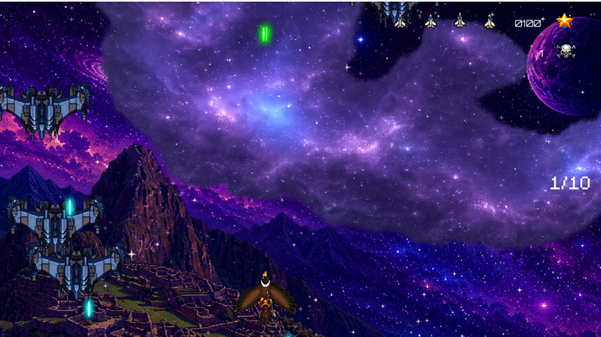
\includegraphics[width=0.6\textwidth]{sistema-de-disparos.png}
    \caption{Sistema de disparo dual del jugador}
    \label{fig:disparos}
\end{figure}

\section{Sistema de Enemigos}

\subsection{Jerarquía de Clases}
Los enemigos utilizan herencia de scripts para compartir comportamiento común:

\begin{figure}[H]
    \centering
    \begin{minipage}{0.6\textwidth}
    \small
    \begin{verbatim}
Enemy.gd (clase base)
    armor = 4 (golpes para destruir)
    Disparo automatico via ShootTimer
    Colisiones con bullet y player
    Explosion al morir
    
    +-- EnemyBlue.gd (movimiento ondulante)
    |     wave_height = 120
    |     wave_speed = 2
    |     horizontal_speed = 120
    |     Movimiento: seno() + rebote en bordes
    |
    +-- EnemyRed.gd (caida vertical rapida)
          velocity.y = aleatorio(250, 1000)
          Caida recta hacia abajo
    \end{verbatim}
    \end{minipage}
    \caption{Jerarquía de herencia de scripts de enemigos}
    \label{fig:herencia}
\end{figure}

\begin{figure}[H]
    \centering
    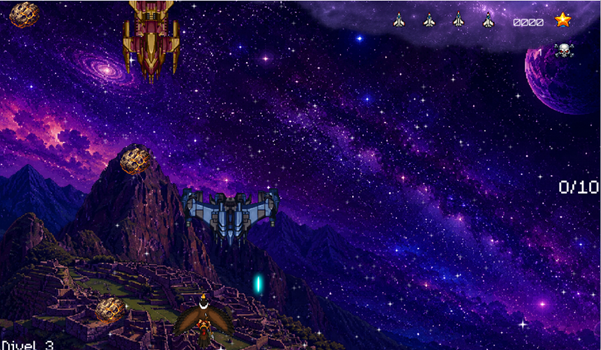
\includegraphics[width=0.6\textwidth]{sistema-de-enemigos.png}
    \caption{Variedad de enemigos y meteoritos en el juego}
    \label{fig:enemigos}
\end{figure}

\subsection{Enemigo Base (\texttt{Enemy.gd})}
El enemigo base define el comportamiento común: sistema de armadura, disparo automático, colisiones y explosión:

\begin{lstlisting}[style=gdscript, caption=Clase base de enemigos]
extends Area2D

export (PackedScene) var EnemyBullet
export var velocity = Vector2(0, 100)
export var armor = 4

func _on_Enemy_area_entered(area):
    if area.is_in_group("bullet"):
        armor -= 1
        area.queue_free()
    elif area.is_in_group("player"):
        armor = 0
    
    if armor <= 0:
        if get_parent().has_method("add_score"):
            get_parent().add_score(100)
        _spawn_explosion()
        # Animacion de muerte...
        queue_free()
\end{lstlisting}

\begin{figure}[H]
    \centering
    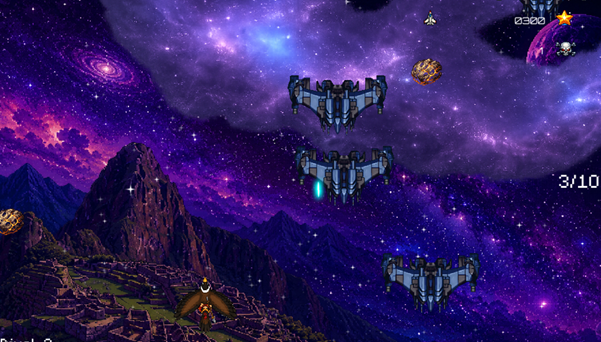
\includegraphics[width=0.6\textwidth]{sistema-de-colisiones.png}
    \caption{Detección de colisiones entre proyectiles y enemigos}
    \label{fig:colisiones}
\end{figure}

\subsection{Enemigo Azul (\texttt{EnemyBlue.gd})}
El enemigo azul se desplaza horizontalmente mientras oscila verticalmente siguiendo una función senoidal:

\begin{lstlisting}[style=gdscript, caption=Movimiento ondulante del enemigo azul]
func _physics_process(delta):
    time += delta
    position.x += velocity.x * delta
    position.y = start_y + sin((time + offset) * wave_speed) * wave_height
    
    # Rebote en bordes
    if position.x <= 64:
        velocity.x = abs(velocity.x)
    if position.x >= Utils.view_size.x - 64:
        velocity.x = -abs(velocity.x)
\end{lstlisting}

\subsection{Enemigo Rojo (\texttt{EnemyRed.gd})}
El enemigo rojo implementa una caída vertical con velocidad aleatoria:

\begin{lstlisting}[style=gdscript, caption=Movimiento del enemigo rojo]
extends "res://Enemy/Enemy.gd"

func _ready():
    randomize()
    velocity = Vector2(0, rand_range(250, 1000))
\end{lstlisting}

\section{Sistema de Meteoritos}

Los meteoritos caen verticalmente y pueden ser destruidos por las balas del jugador (50 puntos cada uno):

\begin{lstlisting}[style=gdscript, caption=Sistema de meteoritos]
extends Area2D

export var speed = 250

func _physics_process(delta):
    position.y += speed * delta
    if position.y > Utils.view_size.y + 50:
        queue_free()

func _on_Meteor_area_entered(area):
    if area.is_in_group("bullet"):
        area.queue_free()
        if get_parent().has_method("add_score"):
            get_parent().add_score(50)
        _spawn_explosion()
        queue_free()
\end{lstlisting}

\section{Sistema de Dificultad Progresiva}

El nivel de dificultad se ajusta dinámicamente en función de la puntuación acumulada, modificando el intervalo de spawn de los enemigos:

\begin{lstlisting}[style=gdscript, caption=Sistema de niveles y dificultad progresiva]
func check_level():
    if score >= 3000:
        level = 3
    elif score >= 1000:
        level = 2
    else:
        level = 1
    apply_level()

func apply_level():
    match level:
        1:
            $SpawnerEnemy/SpawnTimer.wait_time = 2.0
        2:
            $SpawnerEnemy/SpawnTimer.wait_time = 1.2
        3:
            $SpawnerEnemy/SpawnTimer.wait_time = 0.6
\end{lstlisting}

\begin{figure}[H]
    \centering
    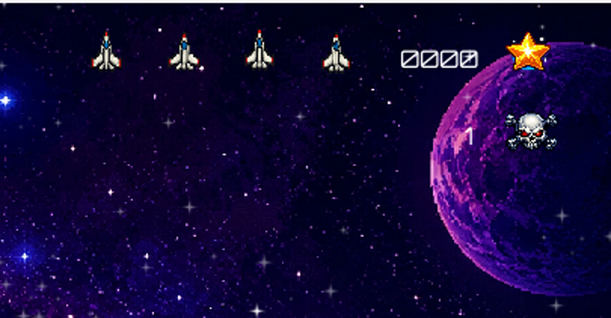
\includegraphics[width=0.6\textwidth]{sistema-de-puntaje.png}
    \caption{Sistema de puntuación y dificultad progresiva}
    \label{fig:puntaje}
\end{figure}

\section{Interfaz de Usuario (HUD)}

El HUD se implementa mediante nodos \texttt{CanvasLayer} que se renderizan sobre la escena de juego, lo que garantiza que los elementos de interfaz mantengan su posición independientemente de la cámara:

\begin{figure}[H]
    \centering
    \begin{subfigure}{0.3\textwidth}
        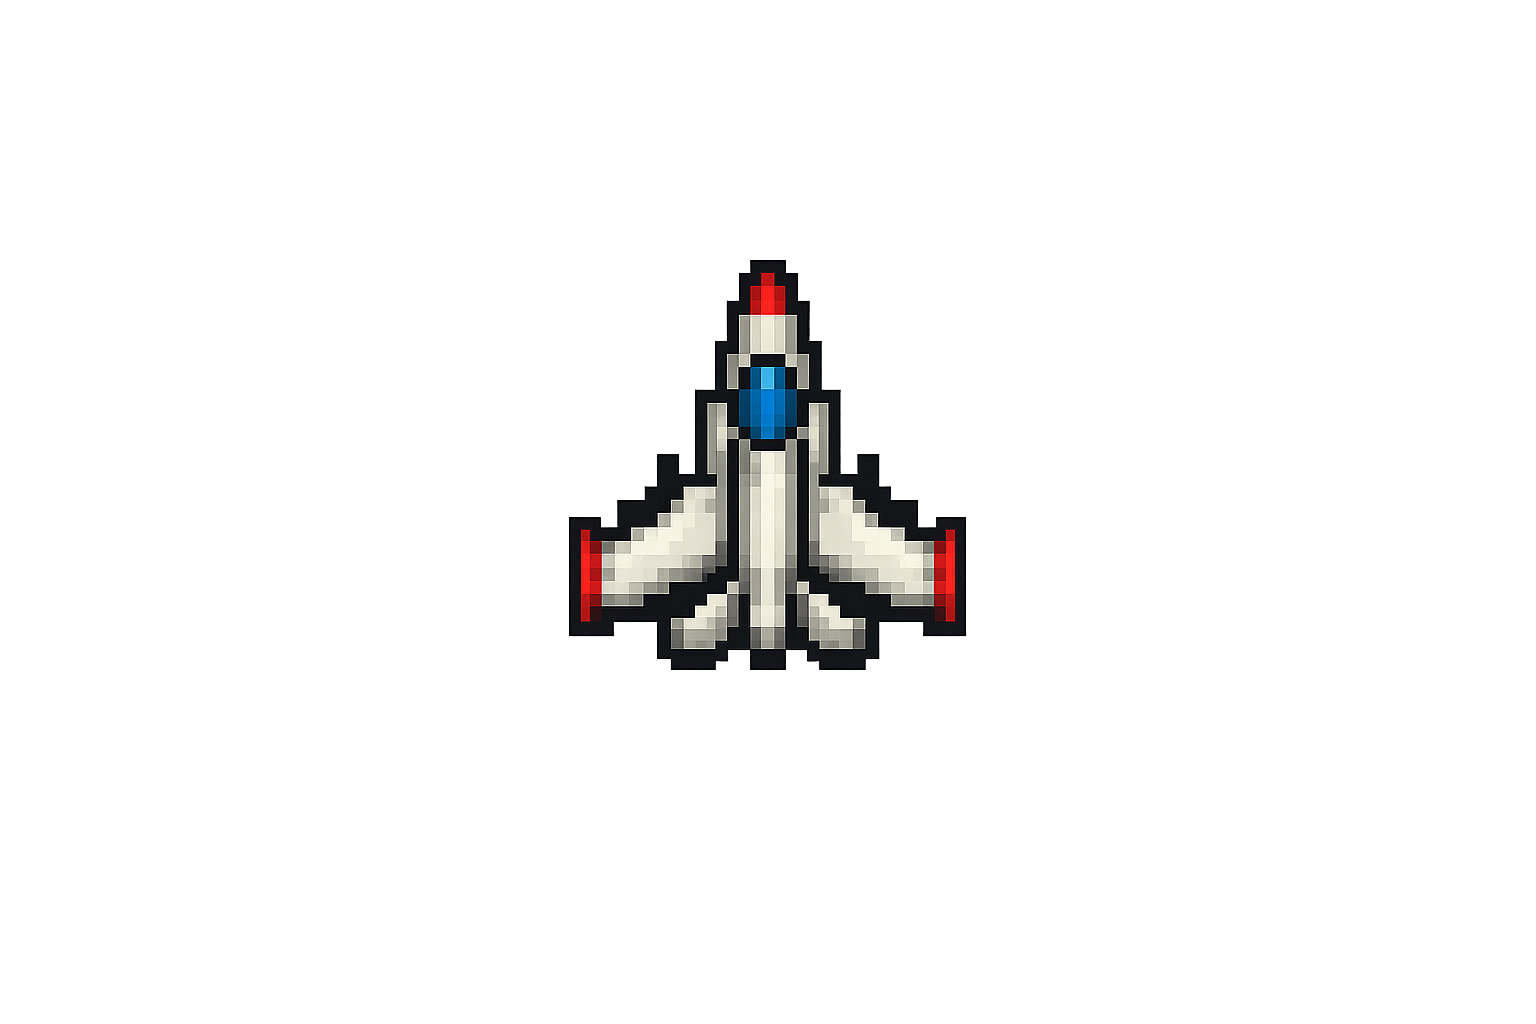
\includegraphics[width=\textwidth]{life_icon.png}
        \caption{Ícono de vida}
    \end{subfigure}
    \begin{subfigure}{0.3\textwidth}
        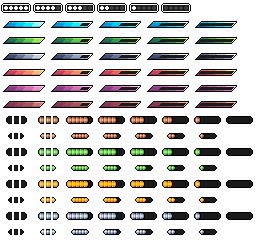
\includegraphics[width=\textwidth]{shield_bar.png}
        \caption{Barra de escudo}
    \end{subfigure}
    \begin{subfigure}{0.3\textwidth}
        
\includegraphics[width=\textwidth]{shield.png}
        \caption{Ícono de escudo}
    \end{subfigure}
    \caption{Elementos del HUD del juego}
    \label{fig:hud}
\end{figure}

\begin{figure}[H]
    \centering
    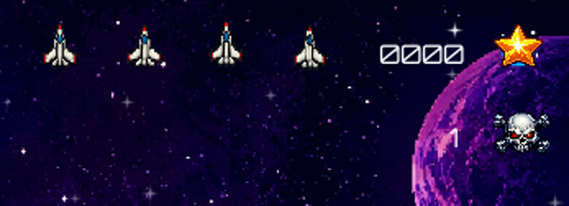
\includegraphics[width=0.5\textwidth]{sistema-de-vidas.png}
    \caption{Sistema de vidas y HUD del juego}
    \label{fig:vidas}
\end{figure}

El HUD incluye:
\begin{itemize}
    \item Indicadores de vidas (4 corazones)
    \item Barra de escudo (5 frames que muestran el progreso de recarga)
    \item Puntuación numérica (4 dígitos)
    \item Indicador de nivel (1-3)
    \item Contador de enemigos destruidos/total ("X/50")
    \item Pantalla de Game Over (overlay rojo con opciones)
\end{itemize}

\begin{figure}[H]
    \centering
    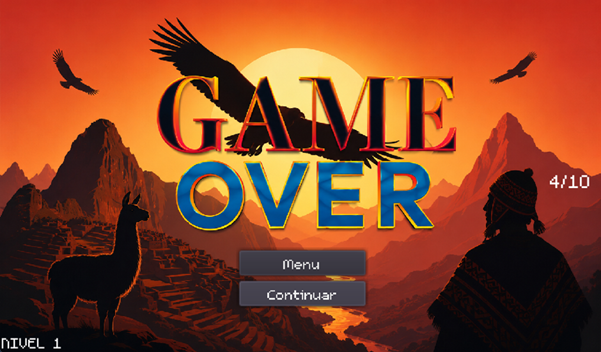
\includegraphics[width=0.5\textwidth]{game-over.png}
    \caption{Pantalla de Game Over}
    \label{fig:gameover}
\end{figure}

\section{Pantalla de Victoria y Progresión}

Al destruir 50 enemigos, el juego carga la pantalla de victoria (\texttt{DefenseCompleted.tscn}) que permite avanzar al siguiente nivel o regresar al menú:

\begin{figure}[H]
    \centering
    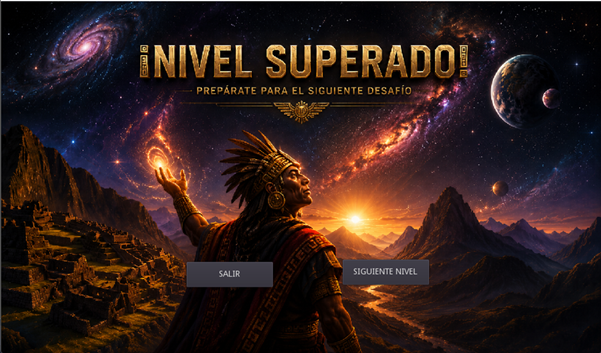
\includegraphics[width=0.6\textwidth]{nivel-superado.png}
    \caption{Pantalla de nivel superado}
    \label{fig:nivelsuperado}
\end{figure}

\begin{figure}[H]
    \centering
    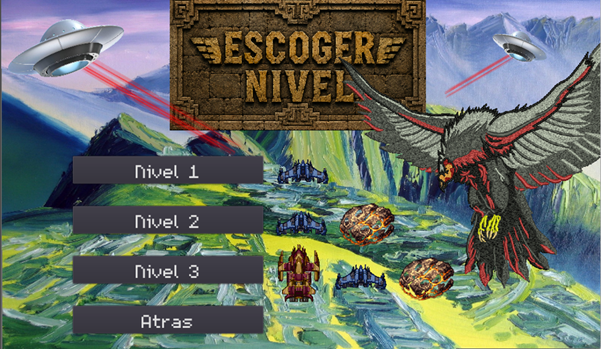
\includegraphics[width=0.6\textwidth]{implementacion-de-niveles.png}
    \caption{Implementación de los tres niveles del juego}
    \label{fig:niveles}
\end{figure}

\begin{lstlisting}[style=gdscript, caption=Progresión entre niveles]
func _on_Siguiente_pressed():
    if Globals.current_stage == 1:
        Globals.current_stage = 2
        get_tree().change_scene("res://stage/Stage2.tscn")
    elif Globals.current_stage == 2:
        Globals.current_stage = 3
        get_tree().change_scene("res://stage/Stage3.tscn")
\end{lstlisting}

\newpage

% ============================================================
% 7. PRINCIPIOS DE CALIDAD TOTAL
% ============================================================
\chapter{Principios de Calidad Total}

La aplicación de los principios de calidad total, basados en las teorías de Edwards Deming \cite{deming1986}, en el desarrollo de \textit{Defensa Cóndor} se manifiesta en los siguientes aspectos:

\section{Mejora Continua (Kaizen)}

El proceso de desarrollo del juego fue iterativo: cada funcionalidad fue prototipada, probada y refinada antes de integrarse al producto final. Por ejemplo, el sistema de escudo pasó por tres iteraciones: inicialmente era una barra que absorbía todo el daño, luego se cambió a un sistema de tiempo de recarga fijo, y finalmente se implementó la versión actual con recarga progresiva y protección condicional.

\section{Enfoque en el Usuario}

La experiencia del jugador fue el centro del diseño. Esto se refleja en:
\begin{itemize}
    \item \textbf{Soporte para gamepad}: se implementó configuración dinámica de botones para garantizar la accesibilidad desde diferentes dispositivos.
    \item \textbf{Retroalimentación visual y auditiva}: cada acción del jugador tiene una respuesta inmediata (sonidos de disparo, daño, escudo; animaciones de explosión; overlay de daño).
    \item \textbf{Curva de dificultad ajustable}: el sistema de niveles progresivos evita la frustración inicial y mantiene el desafío.
\end{itemize}

\section{Gestión de Procesos}

El desarrollo siguió un flujo de trabajo estructurado:
\begin{enumerate}
    \item \textbf{Diseño}: definición de mecánicas, historia y arte conceptual.
    \item \textbf{Prototipado}: implementación rápida de las mecánicas básicas (movimiento, disparo).
    \item \textbf{Desarrollo iterativo}: adición incremental de características (enemigos, escudo, meteoritos).
    \item \textbf{Pruebas}: verificación de colisiones, balance de dificultad y rendimiento.
    \item \textbf{Documentación}: creación de README.md y comentarios en el código.
\end{enumerate}

\section{Prevención de Defectos}

Se implementaron prácticas de prevención de errores:
\begin{itemize}
    \item \textbf{Validación de referencias}: uso de \texttt{is\_instance\_valid()} y \texttt{get\_node\_or\_null()} para evitar errores por nodos faltantes.
    \item \textbf{Limpieza de memoria}: los objetos fuera de pantalla se eliminan automáticamente mediante \texttt{VisibilityNotifier2D} y verificaciones de posición.
    \item \textbf{Manejo de estados}: el juego utiliza variables de estado (\texttt{can\_move}, \texttt{can\_shoot}, \texttt{shield\_recharging}) para prevenir acciones inconsistentes.
\end{itemize}

\section{Toma de Decisiones Basada en Datos}

Durante el desarrollo, se realizaron pruebas de juego para ajustar parámetros:
\begin{itemize}
    \item \textbf{Velocidad de disparo}: ajustada para equilibrar la dificultad.
    \item \textbf{Tiempo de recarga del escudo}: establecido en 10 segundos tras pruebas de usabilidad.
    \item \textbf{Umbrales de nivel}: 1000 y 3000 puntos como puntos de inflexión de dificultad.
\end{itemize}

\newpage

% ============================================================
% 8. CONCLUSIONES
% ============================================================
\chapter{Conclusiones}

El desarrollo de \textit{Defensa Cóndor} como proyecto final de curso permitió alcanzar las siguientes conclusiones:

\begin{enumerate}
    \item \textbf{Godot Engine es una plataforma viable para el desarrollo de videojuegos 2D}: su sistema de escenas y nodos, combinado con GDScript, permitió un desarrollo ágil y estructurado del proyecto. La curva de aprendizaje del motor es accesible para desarrolladores con experiencia previa en programación orientada a objetos.

    \item \textbf{La arquitectura basada en herencia de scripts facilita la extensibilidad}: la implementación de \texttt{EnemyBlue.gd} y \texttt{EnemyRed.gd} como extensiones de \texttt{Enemy.gd} demostró que la herencia permite reutilizar código y añadir nuevas variantes de enemigos con un esfuerzo mínimo (8 líneas para \texttt{EnemyRed.gd}).

    \item \textbf{El sistema de escudo regenerable introduce profundidad estratégica}: la mecánica de protección condicional (solo cuando está al 100\%) obliga al jugador a gestionar el riesgo, añadiendo una capa de decisión más allá del simple reflejo.

    \item \textbf{El soporte para gamepad mejora significativamente la accesibilidad}: la implementación del sistema de control mediante gamepad, con asignación dinámica de botones a través de \texttt{InputMap}, amplía el público objetivo del juego y mejora la experiencia de juego.

    \item \textbf{La gestión de memoria y recursos es crítica en Godot}: la eliminación de instancias fuera de pantalla mediante \texttt{VisibilityNotifier2D} y las comprobaciones de posición son esenciales para mantener un rendimiento estable, especialmente en niveles con múltiples enemigos y proyectiles simultáneos.

    \item \textbf{La dificultad progresiva basada en puntuación es efectiva}: el sistema que ajusta el intervalo de spawn de enemigos según la puntuación acumulada genera una curva de dificultad natural que mantiene al jugador en un estado de \textit{flow} sin necesidad de configuración manual.

    \item \textbf{Trabajo futuro}: el proyecto presenta oportunidades de mejora, como la implementación de power-ups, un sistema de guardado de puntuaciones máximas, una pantalla de pausa dedicada, y la conversión de archivos de audio WAV a OGG para reducir el tamaño del repositorio.
\end{enumerate}

\newpage

% ============================================================
% 9. RECOMENDACIONES
% ============================================================
\chapter{Recomendaciones}

A partir del desarrollo del presente proyecto, se formulan las siguientes recomendaciones para trabajos futuros:

\begin{enumerate}
    \item \textbf{Implementar nuevos niveles} con una mayor variedad de enemigos y obstáculos para incrementar la dificultad y rejugabilidad del videojuego.

    \item \textbf{Incorporar un sistema de guardado de partidas} y una tabla de puntuaciones máximas para mejorar la experiencia del usuario y fomentar la competencia.

    \item \textbf{Agregar nuevos escenarios} inspirados en otros departamentos del Perú con el propósito de continuar promoviendo la riqueza cultural del país.

    \item \textbf{Optimizar el videojuego para dispositivos móviles} y otras plataformas compatibles con Godot Engine, ampliando así su alcance.

    \item \textbf{Incorporar efectos visuales adicionales}, como partículas, iluminación dinámica y animaciones más elaboradas, para mejorar la calidad gráfica del videojuego.

    \item \textbf{Implementar power-ups} que otorguen habilidades temporales al jugador (disparo triple, escudo invulnerable, velocidad aumentada) para añadir variedad estratégica.

    \item \textbf{Agregar una pantalla de pausa dedicada} con opciones de configuración de audio y controles.
\end{enumerate}

\newpage

% ============================================================
% 10. BIBLIOGRAFÍA
% ============================================================
\chapter{Bibliografía}

\begin{thebibliography}{99}

\bibitem[Adams(2014)]{adams2014}
Adams, E. (2014). \textit{Fundamentals of Game Design} (3.ª ed.).
New Riders.

\bibitem[Deming(1986)]{deming1986}
Deming, W. E. (1986). \textit{Out of the Crisis}. MIT Press.

\bibitem[Linietsky y Manzur(2020)]{godot_docs}
Linietsky, J. y Manzur, A. (2020). \textit{Godot Engine Documentation}.
Godot Foundation. \url{https://docs.godotengine.org/}

\bibitem[Nystrom(2014)]{nystrom2014}
Nystrom, R. (2014). \textit{Game Programming Patterns}. Genever Benning.
\url{https://gameprogrammingpatterns.com/}

\bibitem[Schell(2019)]{schell2019}
Schell, J. (2019). \textit{The Art of Game Design: A Book of Lenses} (3.ª ed.).
CRC Press.

\bibitem[UNESCO(2024)]{unesco}
UNESCO. (2024). \textit{Historic Sanctuary of Machu Picchu}.
\url{https://whc.unesco.org/en/list/274/}

\bibitem[bdragon1727(2024)]{bdragon_smoke}
bdragon1727. (2024). \textit{Free Smoke FX Pixel 2} [Paquete de sprites].
itch.io. \url{https://bdragon1727.itch.io/free-smoke-fx-pixel-2}

\bibitem[bdragon1727(2024)]{bdragon_explosion}
bdragon1727. (2024). \textit{200 Pixel Shader Explos and Power} [Paquete de sprites].
itch.io. \url{https://bdragon1727.itch.io/200-pixel-shader-explos-and-power}

\bibitem[bdragon1727(2024)]{bdragon_bullet1}
bdragon1727. (2024). \textit{500 Pixel Bullet 24x24} [Paquete de sprites].
itch.io. \url{https://bdragon1727.itch.io/500-pixel-bullet-24x24}

\bibitem[bdragon1727(2024)]{bdragon_bullet3}
bdragon1727. (2024). \textit{Pixel Bullet 24x24 Part 3} [Paquete de sprites].
itch.io. \url{https://bdragon1727.itch.io/pixel-bullet-24x24-part-3}

\bibitem[bdragon1727(2024)]{bdragon_healthbar}
bdragon1727. (2024). \textit{Basic Pixel Health Bar and Scroll Bar} [Paquete de sprites].
itch.io. \url{https://bdragon1727.itch.io/basic-pixel-health-bar-and-scroll-bar}

\bibitem[Glionox(2024)]{glionox}
Glionox. (2024). \textit{Items 16} [Paquete de sprites].
itch.io. \url{https://glionox.itch.io/items16}

\bibitem[DanteWreckmen(2019)]{dante_weapons}
DanteWreckmen-999. (2019). \textit{Halo Series Master Weapons Pack Sprite Sheet}.
DeviantArt. \url{https://www.deviantart.com/dantewreckmen-999/art/Halo-Series-Master-Weapons-Pack-Sprite-Sheet-553343608}

\end{thebibliography}

\end{document}
